\documentclass[a4paper]{article}
\usepackage{amsmath}
\usepackage{graphicx}
\usepackage{multicol}
\usepackage{tocloft}

\usepackage{geometry}
 \geometry{
 a4paper,
 total={170mm,257mm},
 left=20mm,
 top=10mm,
 bottom=30mm
 }

\begin{document}

\title{EPFL Machine Learning - Project 2}
\author{
  Pierre-Alexandre Lee, Thomas Garcia, Yves Lamonato\\
  \textit{EPFL Lausanne, Switzerland}
}
\date{\vspace{-5ex}}

\maketitle
\mbox{}\\


%=================================================================================================================
%=================================================================================================================


\section{Introduction}
For this project, we will put into practice some of the concepts seen during the lectures. 
Among the proposed projects, we choose the one that involves creating a recommender system from user's ratings of certain products. 
We can find such systems in big online stores like Amazon for example. Ours will be a much simplified version of it of course.  

Just like in the first project, we will use the dataset provided on the Kaggle competition. We have used some libraries, the instruction for their installation can be found in the README.



%=================================================================================================================
%=================================================================================================================



\section{The dataset}
\subsection{Raw data}
The dataset on Kaggle is a .csv file, were each line consist of the matrix coordinates along with the value at those coordinates. Each value is the rating of a certain user (row) for an item (column). The coordinates were given in a String format, like for example \textit{r36\_c124}, which correspond to the 36th row of the 124th column. 
For some of the data processing we used functions from the lab 10 correction, with changes when needed.

\subsection{Data pre-processing}
\begin{enumerate}
\item \textit{Importing data} : With almost all our algorithms, we needed the data to be in a matrix form. We used the sparse format from the Scipy library for efficiency. The loading algorithm reads the .csv file line by line, split the row and column index and subtracts 1 to them (since the indexes of the file begin at 1). We then use those coordinates to fill the sparse matrix with the corresponding ratings.

\item \textit{Exploring the data} : Our data consist of 1'176'952 ratings given by 10'000 users for 1'000 items (almost 11.77\% of the possible ratings). Using some statistics we got from the data importation part, we can plot the number of ratings per user, and also per item (number of ratings given to that item). From those stats, we found that each user in our data has rated at least 3 items, and that each items has at least 8 reviews. This means that we won't have to drop useless users or items. 
\end{enumerate}

\begin{figure}[h]
  \centering
  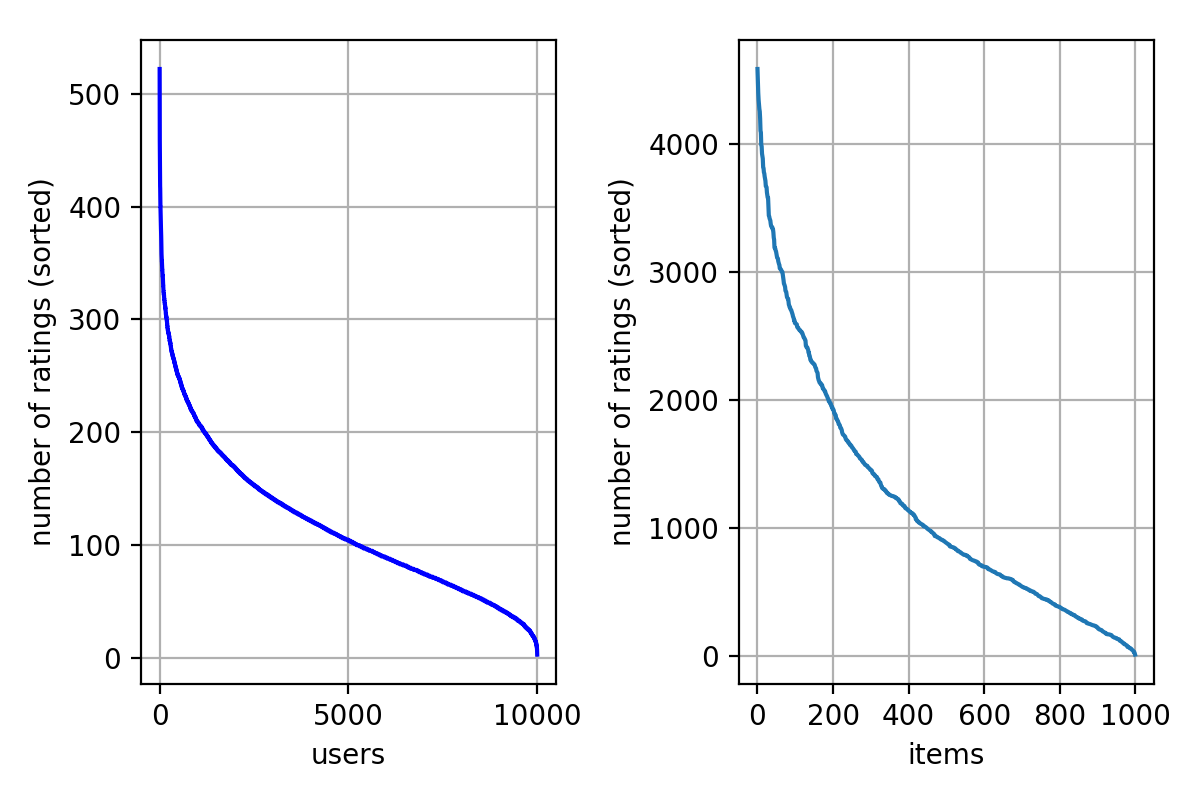
\includegraphics[width=8cm]{stat_ratings.png}
  \label{fig:figure 1}
  \caption{(Left) Sorted number of ratings per user. (Right) Sorted number of ratings for each item.}
\end{figure}

%=================================================================================================================
%=================================================================================================================


\section{Models}
For the SGD and ALS training algorithms, we used the correction of the lab 10 as a template.

\subsection{Models used}
Those models were tested (the results are displayed in a table in the "Results" section):

\begin{itemize}
\item \textbf{Stochastic gradient descent (SGD):}  

This method, while quite simple, was too slow, and we didn't get very good results.
The used a parameter \textit{gamma}=0.02 (found via grid search) and a number of epochs=20 (with a higher number of epochs the error only improved marginally).
\item \textbf{Alternating least squares with bias estimation (ALS):}  

For this model, we tested both the standard version from lab 10 and one where we also took into consideration the bias of the ratings. For the last one we computed the average of all ratings, the average rating per user and then the average rating per item. Those fixed values were included in the computation of the new features for users and items, and we adapted our error and results-exporting functions to take it into account.  
\paragraph{}
While one could think the best bias estimation wouldn't consider the empty entries of the ratings sparse matrix, we had better results by taking them for the global, user and item mean (thus our means were often small).
\paragraph{}
We got our best result from the version with bias. For the two of them, we took for the stopping criterion the point where the training rmse change would be less than 1e-05. We observed from the error plots below (see figures 3 and 4) that lowering the criterion would only marginally improve the result for a much greater computation time. 
\item \textbf{external library \textit{Nimfa}:}  

The Nimfa library wasn't really good, because it isn't intended for recommendation systems, but more for pure matrix factorization. It even didn't let us specify a \(\lambda\) parameter.
\item \textbf{external library \textit{pyspark.mllib}:}  

This library gave us our best results, and it was quite fast (but to get our final result we had to let it run for 40 minutes on one average laptop).
For our result, we set the number of iterations (a parameter of the ALS model from spark, which determine the number of passes through the dataset) to 250. Setting it to a higher value only increased the time for a marginally better result. 
\end{itemize}

\paragraph{}
For each model, there was two or three basic parameters : The \textit{rank} of the approximation (K in the lecture notes) and the \(\lambda\) of the regularization, with sometimes one for the users and one for the items. 

\paragraph{}
Those parameters were tweaked using grid search. For each model, we noticed that the best \textit{rank} was usually around 100 : 
More would lead to the training error decreasing, but the testing error would increase as the result of overfitting. Using a lower \textit{rank} would result in both the training and testing error increasing.
\paragraph{}
For the regularization parameter \(\lambda\), we noticed that a good value was 0.09 for this data. We also noticed that when a \(\lambda_{user}\) and a \(\lambda_{item}\) could be specified separately, we could have good result in setting \(\lambda_{user} = 0.28\) and \(\lambda_{item} = 0.028\), with the \(\lambda_{user}\) being 10 times higher than the \(\lambda_{item}\). We think this can be explained by the fact that there are 10 times less users than item. 
\paragraph{}
However, our best results were obtained using the same \(\lambda = 0.09\) for both the users and the items, even though some of our libraries, for example \textit{pyspark.mllib}, which only takes one \(\lambda\) parameter, says in its documentation that it also scales the parameter accordingly for the users and the items.

\subsection{Cross-validation}
We decided not to do any kind of cross-validation, since each run of most algorithms already takes at least 25 minutes, sometimes much longer.
Also, the score we got in local for the test data (10\% of the whole thing) is consistent with what we get on kaggle.

\subsection{Model accuracy}
For the computation of the error, we used the \textit{RMSE} over the given entries. This is also what is used in the Kaggle competition.  
$$ RMSE(W, Z) := \sqrt{\frac{1}{|\Omega|} \sum\nolimits_{(d, n) \in \Omega} [\textit{x\textsubscript{dn}} - (WZ^\top)\textsubscript{\textit{dn}}]^2} $$
Where \(\Omega\) is the set of all our given entries in the ratings matrix, \(W\) is the feature matrix of the users (dimension 10000 x K) and \(Z\) the feature matrix of the items (dimension 1000 x K).



%=================================================================================================================
%=================================================================================================================



\section{Results}
We give here our best results for each model.
While in local the ALS with bias is the best, on the kaggle competition, Spark is a little bit better. We also couldn't get any graph for Spark since we can't access the error during the computation.
\mbox{}\\
\begin{figure}[h]
  \centering
  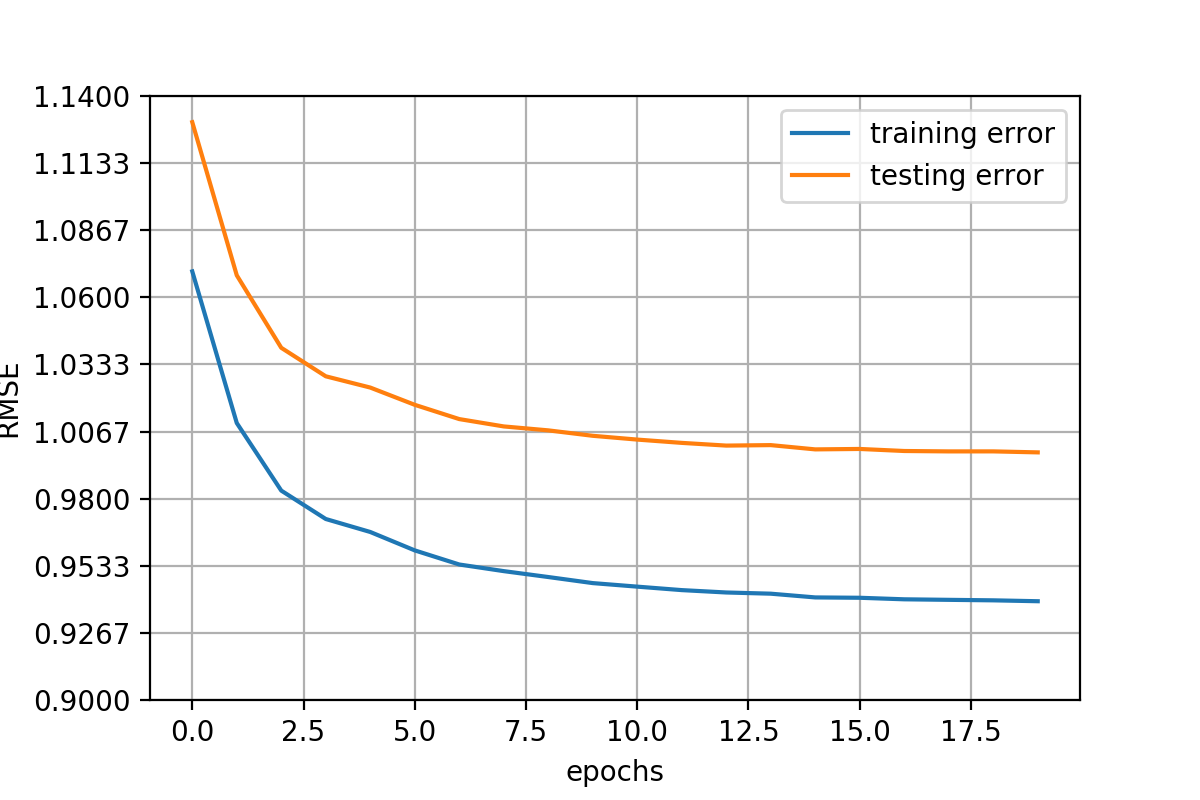
\includegraphics[width=8cm]{RMSE_SGD.png}
  \caption{RMSE for the SGD model}
  \label{fig:figure 2}
\end{figure}

\mbox{}\\

\begin{figure}[h]
  \centering
  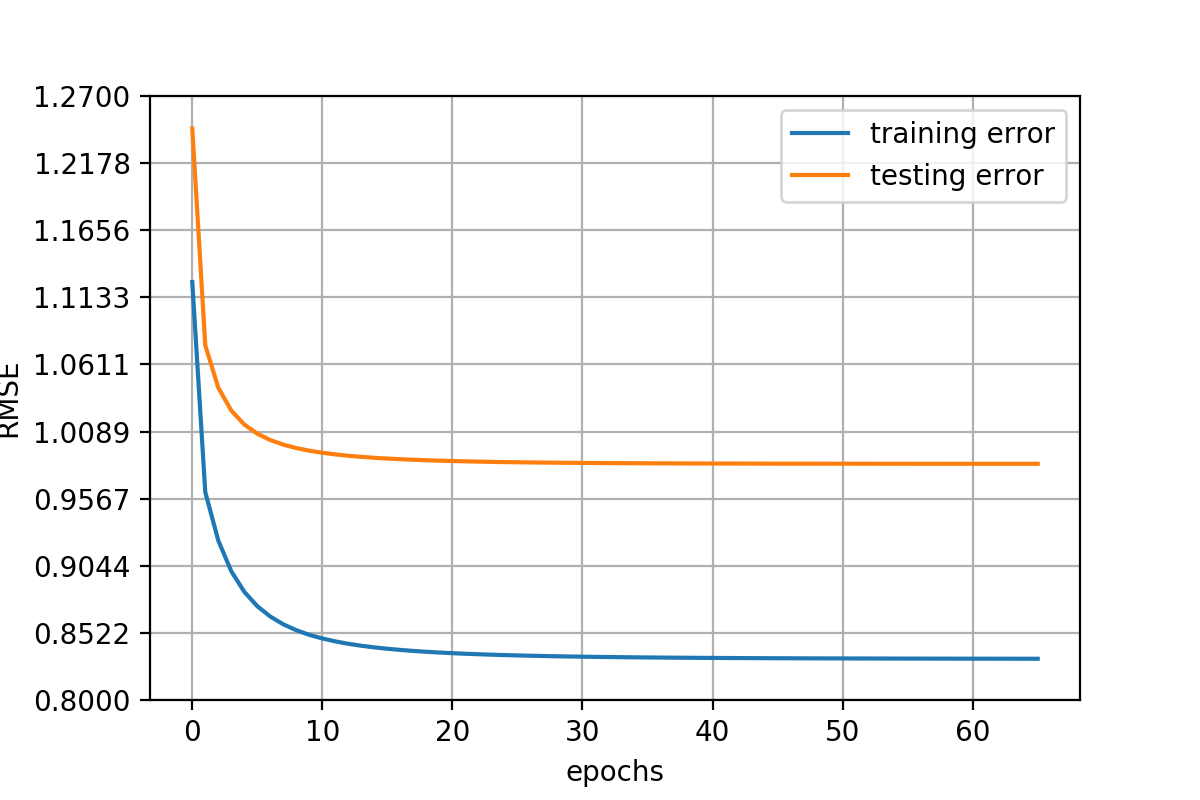
\includegraphics[width=8cm]{RMSE_ALS.png}
  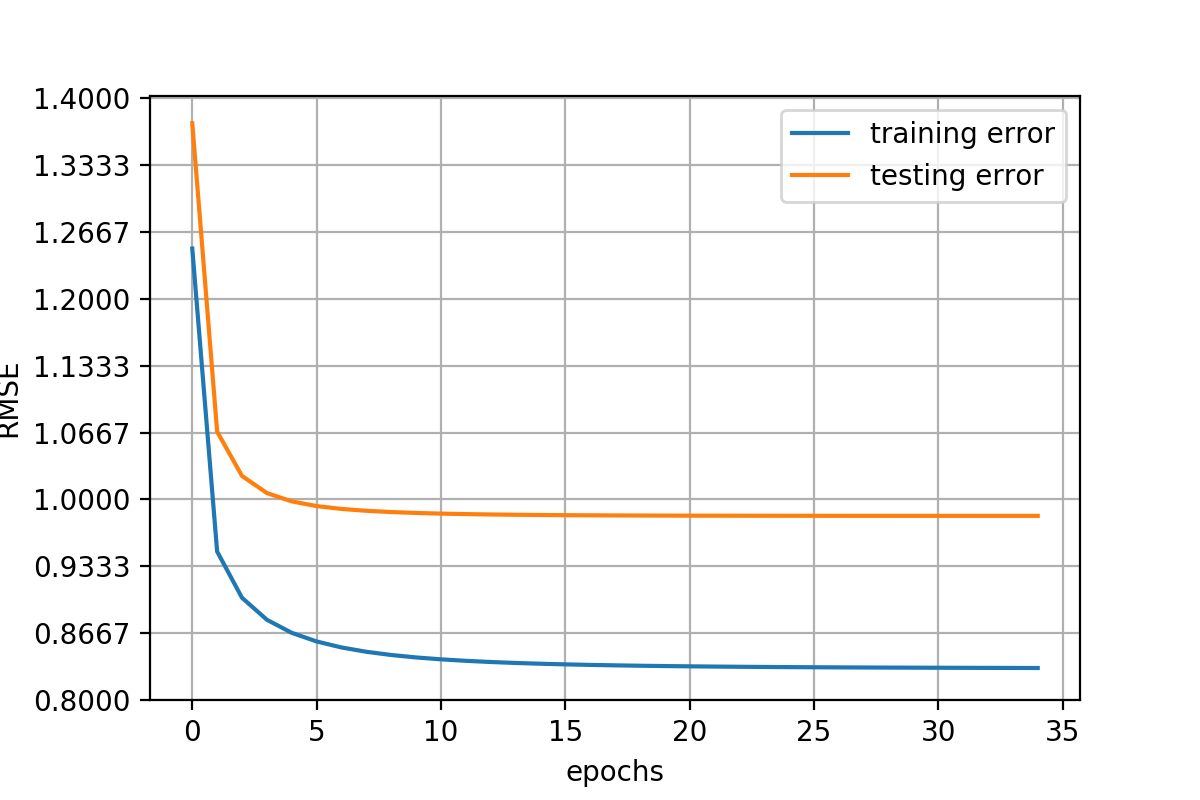
\includegraphics[width=8cm]{RMSE_ALS_BIAS.png}
  \label{fig:figure 3}
  \caption{(Left) RMSE for the ALS without bias model.}
  \label{fig:figure 4}
  \caption{(Right) RMSE for the ALS with bias model.}
\end{figure}

\mbox{}\\

\begin{table}[h!]
  \centering
  \begin{tabular}{|c|c|c|c|c|}
    \hline
    \textbf{Model} & \textbf{Testing accuracy} & \textbf{\textit{rank}} & \boldmath\(\lambda_{user}\)& \boldmath\(\lambda_{item}\)\\
    \hline
    SGD & 0.99839302 & 100 & 0.09 & 0.09\\
    \hline
    ALS (without bias) & 0.98380363 & 110 & 0.09 & 0.09\\
    \hline
    ALS (with bias) & 0.98358184 & 110 & 0.09 & 0.09\\
    \hline
    Nimfa & 3.48903279 & 100 & / & / \\
    \hline
    pyspark.mllib & 0.98768581 & 100 & 0.09 & 0.09\\
    \hline
  \end{tabular}
  \caption{RMSE and best parameters for our models}
  \label{tab:table 1}
\end{table}
\mbox{}\\
%=================================================================================================================
%=================================================================================================================



\section{Conclusion}
Since most of the work is parameter tuning, we tried many methods and libraries. In the end our self-implemented ALS with bias implementation was the best one (with spark being the close second), although not the fastest (the spark library was very quick, since it used the whole CPU with great parallelization of the task). 

\end{document}
